\documentclass[varwidth=true, border=2pt]{standalone}

\usepackage{pgfplots}
\usepackage{tikz}

\usetikzlibrary{calc,patterns,angles,quotes}

\begin{document}

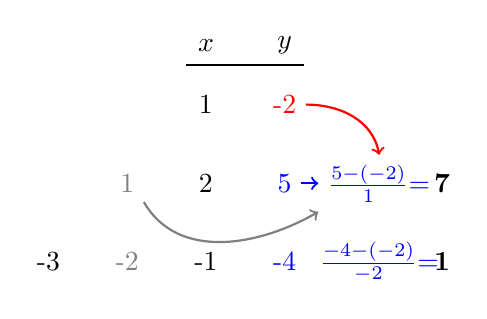
\begin{tikzpicture}
	\node (A) at (1.5,3.25) {$x$};
	\node  (B) at (1.5,2.5){1}; 
	\node (C) at (1.5,1.5) {2};
	\node (D) at (1.5,0.5) {-1};
	\node (E) [gray] at (0.5,1.5) {1};
	\node (F) [gray] at (0.5,0.5) {-2};
	\node (G) at (-0.5,0.5) {-3};
	\node (a) at (2.5,3.25) {$y$};
	\node (b)[red] at (2.5,2.5) {-2};
	\node  (c) [blue] at (2.5,1.5) {5};
	\node  (d) [blue] at (2.5,0.5) {-4};
	\node (e) at (4.5,1.5) {\textbf{7}};
	\node (f) at (4.5,0.5) {\textbf{1}};

	\node(L1)  [blue]  at (3.7,0.5) {$\frac{-4-(-2)}{-2}$=};
	\node (L2) [blue]  at (3.7,1.5) {$\frac{5-(-2)}{1}$=};


	\draw [->, thick, blue] (c) to (L2);
	\draw [->, thick, red] (b.east) to [out=0, in = 100] (L2.north);
	\draw [->, thick, gray] (E.south east) to  [out=300, in = 210] (L2.south west);
	\draw [thick, black] (1.25,3) to (2.75,3);


\small


\normalsize

\end{tikzpicture}
\end{document}